\chapter{Modellare gli agenti di sistema e le loro responsabilità}
Avendo parlato ampiamente dei goal, parliamo degli agenti, ovvero chi ha la responsabilità 
che i goal vengano raggiunti. Non si parla solo di \textbf{responsabilità}, ma anche di 
\textbf{capacità}, ovvero quali sono gli agenti che sono in grado di raggiungere 
i goal, chi ha interesse a raggiungerli e quelli a cui verrà assegnata la responsabilità
del raggiungimento del goal.
\section{Caratteristiche degli agenti di sistema}
\subsection{Capacità degli agenti}
Gli agenti possono \textit{monitorare} o \textit{controllare} delle grandezze 
del sistema, ovvero possono avere la capacità di \textit{osservare} o \textit{modificare}
lo stato del sistema.

\begin{figure}[H]
    \centering
    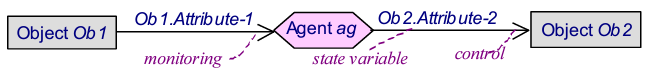
\includegraphics[width=0.7\textwidth]{img/agents.png}
    \caption{Esempio di agenti che monitorano e
    controllano delle grandezze del sistema.}
    \label{fig:agenti}
\end{figure}
\begin{itemize}
    \item In input all'agente abbiamo grandezze 
    che l'agente monitora.
    \item In output all'agente abbiamo grandezze
    che l'agente controlla.
\end{itemize}
Di fatto, quello che gli agenti possono monitorare non sono solo 
dati, ma ogni tipologia di oggetto, ad esempio un agente potrebbe monitorare un 
campo di un oggetto, la presenza di associazioni tra oggetti, ecc.
\subsection{Responsabilità degli agenti}
È importante che una variabile sia controllata da al più un agente, altrimenti
si rischiano conflitti di responsabilità.

\begin{tcolorbox}[colback=violet!5!white,colframe=violet!75!black, title=Responsabilità di un agente]
    La responsabilità di un agente viene rappresentata con un \textbf{responsibility link}, ovvero 
    un collegamento tra l'agente e il goal che l'agente deve raggiungere.
\end{tcolorbox}
\begin{figure}[H]
    \centering
    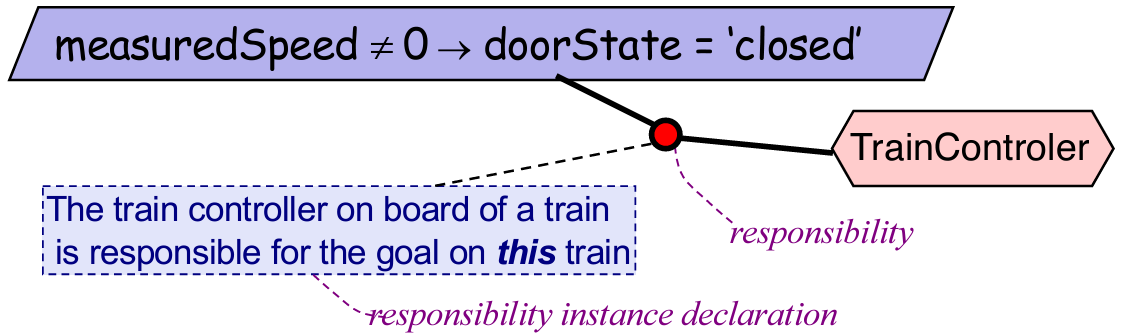
\includegraphics[width=0.7\textwidth]{img/responsibility.png}
    \caption{Esempio di responsabilità di un agente.}
    \label{fig:responsibility}
\end{figure}
\subsubsection{Assegnamento di responsabilità e capacità degli agenti}
L'assegnamento delle responsabilità deve essere subordinato al fatto che l'agente 
possieda le capacità di monitorare e controllare le grandezze necessarie
per il raggiungimento del goal.
Per farlo si definisce una lista di transizioni di stato che l'agente può monitorare e controllare in 
modo che il goal sia soddisfatto.

Un goal potrebbe essere non realizzabile per l'agente quando delle variabili importanti 
non possono essere monitorate o controllate dall'agente stesso. Se ci sono variabili 
di stato che vengono valutate in stati futuri, quando il goal esprime delle 
condizioni istantanee, allora il goal non è realizzabile.
Un'altra condizione si verifica quando il goal non è soddisfacibile sotto determinate 
condizioni, ovvero il goal non è realizzabile in alcune situazioni.
\subsection{Operazioni degli agenti}
Per raggiungere gli obiettivi, gli agenti devono prendere delle decisioni intraprendendo 
delle operazioni.
Fare un'operazione vuol dire che l'agente deve impostare o leggere delle variabili negli 
oggetti che controlla o monitora. Deve farlo nelle condizioni in cui il 
sistema opera.
\begin{figure}[H]
    \centering
    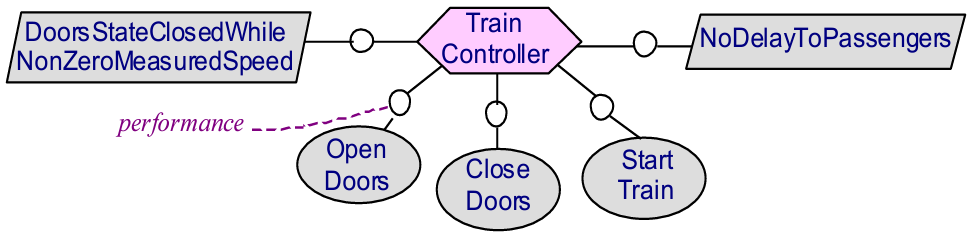
\includegraphics[width=0.7\textwidth]{img/performance.png}
    \caption{Esempio di operazioni di un agente.}
    \label{fig:operations}
\end{figure}

Il collegamento tra l'agente e l'operazione che l'agente deve compiere viene
rappresentato con un \textbf{performance link}.

\subsection{Desideri dell'agente}
Un agente umano potrebbe avere dei desideri, ovvero degli obiettivi personali che
non sono necessariamente in linea con i goal del sistema.

Un esempio di desiderio di un agente umano potrebbe essere ``\textit{Un Patron 
vuole che il periodo di prestito sia lungo}''.

Ci forniscono un modo per guidare l'assegnamento delle responsabilità, in quanto
un agente umano potrebbe avere un desiderio che non è in linea con i goal del sistema.
Pensare ai desideri degli agenti può quindi guidare già in fase di assegnamento 
delle responsabilità.

\subsection{Conoscenza e credenze degli agenti}
È possibile modellare sia la conoscenza che le credenze degli agenti rispetto una 
\textbf{memoria locale} che l'agente possiede rispetto all'ambiente reale.

\begin{itemize}
    \item Un fatto $F$ è creduto dall'agente se $F$ è nella memoria locale dell'agente.
    \item Un fatto $F$ è conosciuto dall'agente se $F$ è nella memoria locale dell'agente e 
    $F$ è vero, proprietà posseduta dall'ambiente o dal sistema.
\end{itemize}
Tale considerazione è importante perché ci permette di fare delle considerazioni sulla 
\textbf{sicurezza}.
\subsection{Dipendenze tra agenti}
Una dipendenza tra due agenti si verifica quando un agente è responsabile del raggiungimento
di un goal, ma un altro agente, per aggiungere un determinato goal 
deve aspettare che il primo agente abbia raggiunto il suo goal.
\begin{figure}[H]
    \centering
    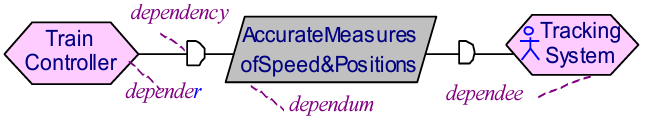
\includegraphics[width=0.7\textwidth]{img/dependent.png}
    \caption{Esempio di dipendenze tra agenti.}
    \label{fig:dependencies}
\end{figure}
Tali dipendenze possono propagarsi a catena. In sistemi critici è opportuno non 
avere catene troppo lunghe.
\section{Rappresentazione della modellazione degli agenti}
\subsection{Agent diagram}
\begin{tcolorbox}[colback=blue!5!white,colframe=blue!75!black, title=Agent diagram]
    L'agent diagram è un diagramma che ha come prospettiva principale gli agenti
    e permette di rappresentare le \textit{responsabilità}, le \textit{capacità} e le
    \textit{operazioni} degli agenti.
\end{tcolorbox}
Possiamo, come nel caso dei goal, possiamo avere degli \texttt{OR}-assignments, ovvero
un goal può essere assegnato a più agenti e il goal è soddisfatto se almeno uno degli
agenti ha raggiunto il goal. Ricordiamoci che ogni goal deve essere assegnato ad un
solo agente, per questo motivo non possiamo avere \texttt{AND}-assignments.
\begin{figure}[H]
    \centering
    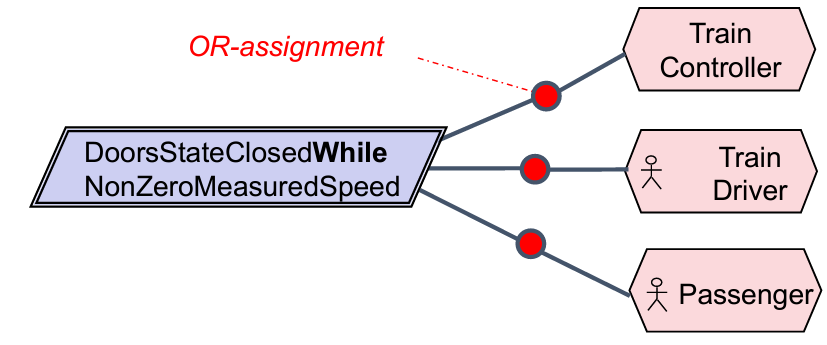
\includegraphics[width=0.7\textwidth]{img/agentdiagram.png}
    \caption{Esempio di \texttt{OR}-assignment in un agent diagram.}
    \label{fig:agentdiagram}
\end{figure}
\subsection{Context diagram}
\begin{tcolorbox}[colback=cyan!5!white,colframe=cyan!75!black, title=Context diagram]
    Il context diagram è una vista che rappresenta solamente la relazione tra variabili 
    \textit{controllate} e \textit{monitorate} dagli agenti.
\end{tcolorbox}
\begin{figure}[H]
    \centering
    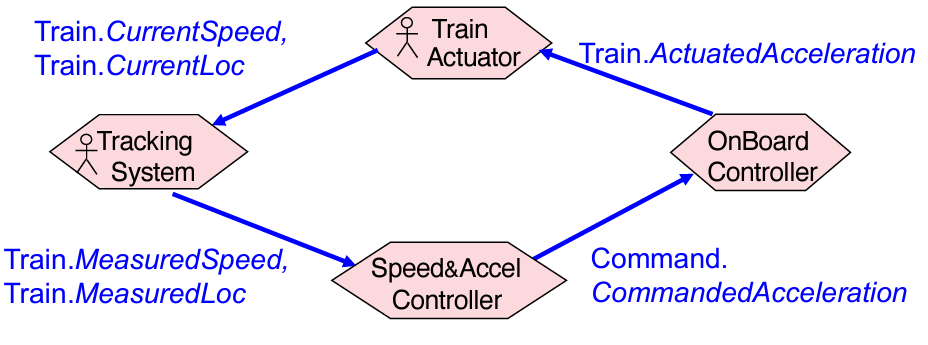
\includegraphics[width=0.7\textwidth]{img/contextdiagram.png}
    \caption{Esempio di context diagram.}
    \label{fig:contextdiagram}
\end{figure}
Un agente potrà prendere decisioni in relazione alle informazioni in termine di 
variabili controllate e monitorate.
\subsection{Dependency diagram}
\begin{tcolorbox}[colback=yellow!5!white,colframe=yellow!75!black, title=Dependency diagram]
    Il dependency diagram è una vista che rappresenta le \textit{dipendenze} tra agenti.
\end{tcolorbox}
\begin{figure}[H]
    \centering
    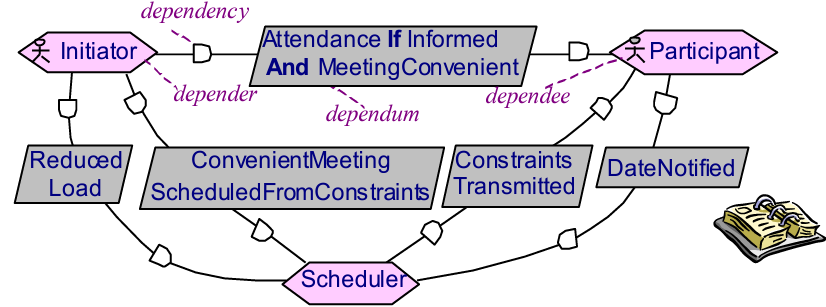
\includegraphics[width=0.7\textwidth]{img/dependencydiagram.png}
    \caption{Esempio di dependency diagram.}
    \label{fig:dependencydiagram}
\end{figure}
\section{Raffinamento e astrazione degli agenti}
Gli agenti possono essere raffinati in sottoagenti, ovvero possiamo avere una
decomposizione gerarchica degli agenti. Questo permette di avere una visione
più dettagliata degli agenti e delle loro responsabilità.
Laddove un goal di alto livello è assegnato ad un agente di alto livello, questo
può essere raffinato in sottoagenti che si occupano di raggiungere i goal di
basso livello rispetto ad una mappatura 1 a 1.

\begin{tcolorbox}
    È importante ricordare che gli agenti sono ruoli e non persone o entità fisiche.
\end{tcolorbox}
\begin{figure}[H]
    \centering
    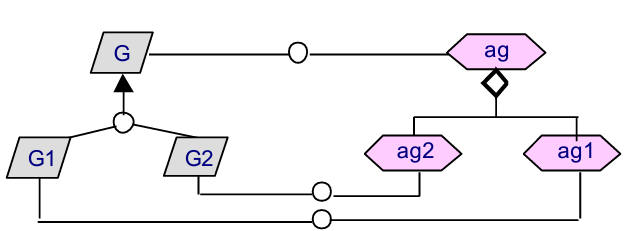
\includegraphics[width=0.7\textwidth]{img/agentraf.png}
    \caption{Esempio di raffinamento di agenti.}
    \label{fig:refinement}
\end{figure}
\section{Euristiche per la modellazione degli agenti}
\begin{itemize}
    \item \textbf{Identificazione degli agenti}: quando si legge la definizione di un goal,
    implicitamente nella definizione c'è il concetto di variabile controllata o monitorata.
    \item Quando leggiamo le \textbf{definizione} possiamo vedere le azioni degli 
    agenti.
    \item  Quando assegniamo una responsabilità ad un agente umano bisogna valutare 
    anche i \textbf{desideri} dell'utente (\textit{i goal di sicurezza informatica devono essere 
    assegnati a persone che hanno a cuore la sicurezza del sistema, quindi in contrasto con 
    il desiderio dell'utente finale}).
    \item Non confondere agenti a livello di prodotto con gli stakeholder a livello 
    di processo. Gli agenti sono dei \textbf{ruoli}, mentre gli stakeholder sono delle
    persone che intervisto, di fatto la stessa persona potrebbe avere ruoli diversi ed 
    essere modellato in agenti diversi.
    \item \textbf{Assegnare responsabilità a componenti software}: per raggiungere 
    un livello di automazione maggiore (\textit{dipende e va valutato in base ai desideri}).
    \item \textbf{Raffinare gli agenti in linea con i goal}: in modo da raggiungere una 
    granularità tale da poter assegnare responsabilità in modo chiaro.
\end{itemize}

\section{Derivare i context diagram dai goal}
Implicitamente i goal possono far riferimento a variabili controllate e monitorate, 
quindi possiamo creare i link che monitora la variabile monitorata e controlla 
la variabile controllata, iterando agente per agente.
\begin{figure}[H]
    \centering
    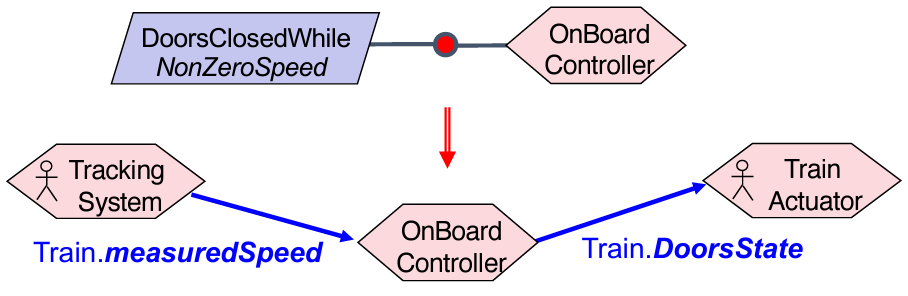
\includegraphics[width=0.7\textwidth]{img/fromgoaltocontext.png}
    \label{fig:contextgoal}
\end{figure}